\documentclass[10pt,a4paper]{article} 
\usepackage[utf8]{inputenc}
\usepackage[ngerman]{babel}
\usepackage{amsmath}
\usepackage{amssymb}
\usepackage{geometry}
\usepackage{hyperref}
\usepackage[table]{xcolor}
\usepackage{wasysym}
\geometry{
  left=3cm,
  right=3cm,
  top=3cm,
  bottom=3cm,
  bindingoffset=0mm
}
\usepackage{graphicx}
\usepackage{dsfont}

\author{Patrick Neher, Ruedi Lüthi}
\title{Thema 4: Stabilität des Golfstroms \\ \textbf{Konzept} }

\begin{document}

	\maketitle

	\subsection*{Offene Fragen}

	Eine erste Studie der Unterlagen hat bei uns bereits viele Fragen aufgeworfen. Somit ist das erste Ziel des Projektes diese Fragen umfänglich zu beantworten, um ein genaues Verständnis für das beschriebene Modell zu erhalten. Ein paar der Unklarheiten möchten wir bereits hier beschreiben:\\
	
	Nach Beschreibung muss \(T^*_1 > T^*_2\) sowie \(S^*_1 < S^*_2\) gelten. So gilt auch \(T^*_{01} > T^*_{02}\) sowie \(S^*_{01} < S^*_{02}\). Damit ist \(T^*_0 = T^*_{01} - T^*_{02} > 0\) und \(S^*_0 = S^*_{01} - S^*_{02} < 0\). Was wiederum bedeutet, dass für \(a, b, c, k_T, s_T > 0\) die Werte \(2\frac{ab}{k_T}T^*_0 = \alpha > 0\) und  \(2\frac{ac}{k_T}S^*_0 = \beta < 0\) gelten muss. Womit wiederum \(\alpha - \beta > 0\) gilt. Betrachten wir nun die Funktion \(g(q) = \alpha \frac{1}{1+|q|} - \beta \frac{\gamma}{\gamma + |q|} \):

	\begin{center}
	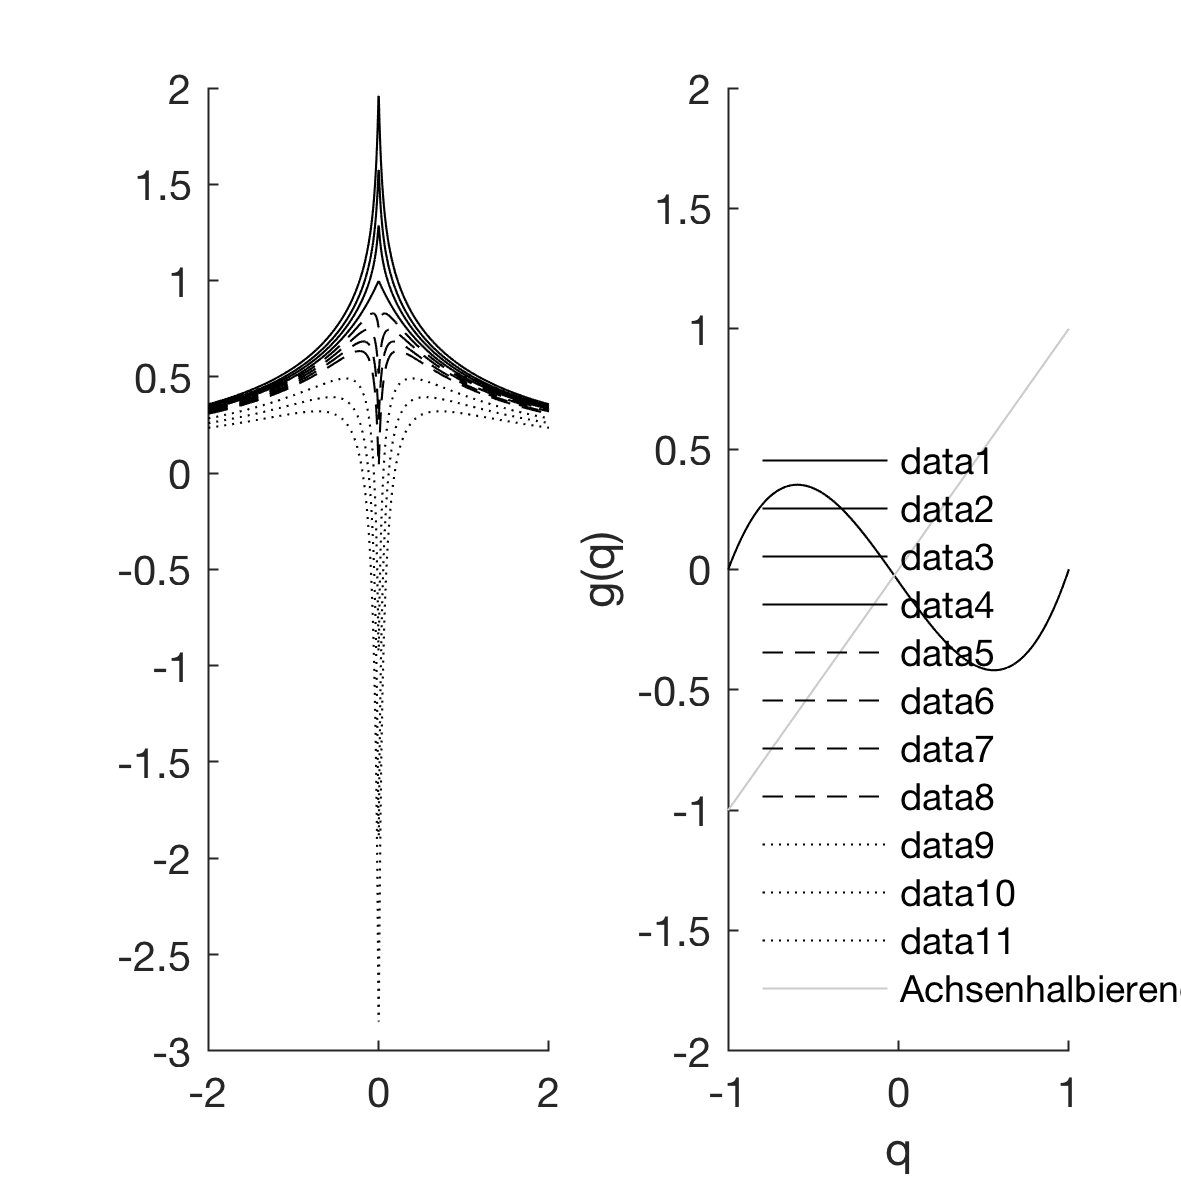
\includegraphics[width=9cm]{Grafik/g_von_q.png} \\
	\textit{Abb. 1 zeigt die Funktion \(g(q)\) für \(\alpha = 1, \gamma = 0.2\) und Variationen für \(\beta\). Dabei ist \(\beta < 0\) für die durchgezogenen Linien, \(\beta > 0\) und \(\alpha - \beta > 0\) für die gestrichelte Linien und \(\beta > 0\) und \(\alpha - \beta < 0\) für die gepunkteten Linien.}
	\end{center}
	
	Wie der Abb. 1 zu entnehmen ist, kann aber die in den Unterlagen beschrieben charakteristische Form (hier gestrichelt und gepunktet) nur für Werte mit \(\beta > 0\) angenommen werden?
	
	Allgemeiner noch, wie ist überhaupt der Graph für die Funktion \(g(q)\) zu deuten? In Worten: \(g(q)\) zeigt die Flussmenge (abhängig von der Flussmenge?) wenn \(T\) und \(S\) im Gleichgewicht sind? Klar ist, dass bei den Schnittpunkten mit der Achsenhalbierenden \(q = g(q)\) sein muss. Also sind bei den Schnittpunkten alle drei Größen \(T,S,q\) im Gleichgewicht? Aber was bedeuten die anderen Punkte auf dem Graphen? Oder die Punkte leicht neben den Schnittpunkte? \\
	
	Wie ist die Äquivalenz von \(g(q)\) und \(k(q)\) zu verstehen?
	\begin{align*}
		q = g(q) &\Rightarrow 0 = q - g(q) \stackrel{q > 0}{=}  q - \left(\alpha \frac{1}{1+q} - \beta \frac{\gamma}{\gamma + q} \right) \\
		& \stackrel{\substack{\textrm{warum}\\\textrm{äquivalent?}}}{\Rightarrow}
		k(q) := \left( q - g(q) \right) (1+q) (\gamma + q) = 0 \\
	\end{align*} \\
	
	Bei der Gleichgewichtsuntersuchung sind ja jeweils \(T^*_{01}, T^*_{02}, S^*_{01}, S^*_{02}\) feste Größen. Jetzt werden aber ja genau diese durch den Fluss des Golfstromes beeinflusst. Um eine Aussage über die Auswirkungen treffen zu können, müssen nun die Werte dieser Größen variiert werden, oder sollen diese Größen auch als Funktion der Zeit beschrieben sein? Denn eigentlich starten man ja mit einer bestimmten Umgebungstemperatur, welche sich aber ja erst durch Klimawandel etc. verändert. \\
	
	Wie wird die Matrix A im Abschnitt 13.4.2 konstruiert?
	
	\newpage
	\subsection*{Parameterwahl}
	
	Um das Modell mit der Realität vergleichen zu können, möchten wir realistische Werte für die Konstanten \( T_0, S_0, k_t, k_s,  a, b, c\) bestimmen.
	
	Für die Umgebungstemperatur \(T_0\) empfiehlt sich folgende Quelle: \url{https://data.giss.nasa.gov/gistemp/}. Dort gibt es historische Jahreswerte zurück bis ins Jahre 1880, sowie Werte zu den einzelnen Monaten eines Jahres. Also könnte damit problemlos auch eine Funktion \(T_0(t)\) interpoliert werden.
	
	Für den Salzgehalt \(S_0\) haben wir als Quelle \url{https://podaac.jpl.nasa.gov/SeaSurfaceSalinity} gefunden. Hier gibt es auch historische Jahreswerte, sowie Werte zu den einzelnen Monaten. Wobei aber eine lokale Bestimmung für Nordmeer und Golf von Mexiko aus den Daten exportiert werden müsste.
	
	Die Größen \(k_T, k_S\) sind physikalische Konstanten und sicherlich einfach zu finden.
	
	Der Wert des Proportionalitätsfaktor \(a\) ist uns noch unklar?
	
	Die Werte für \(b\) und \(c\) für die lineare Approximation der Salzgehalt, Temperatur, Dichte Relation können aus der Abbildung 13.2 in den Unterlagen entnommen werden.
	
	\begin{center}
	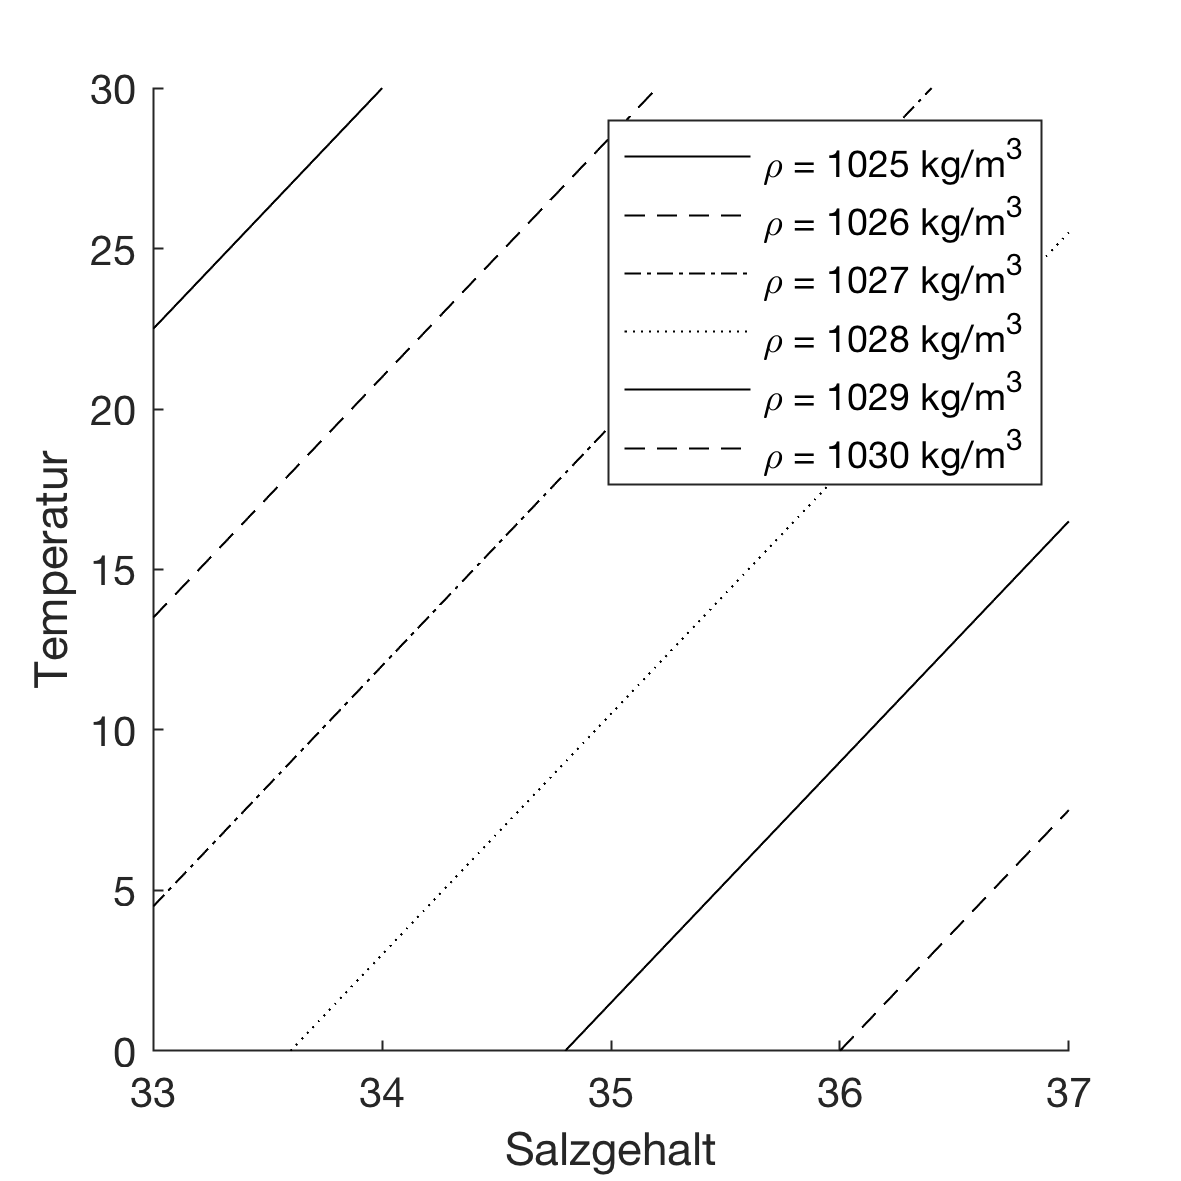
\includegraphics[width=9cm]{Grafik/salz_temp_dichte.png} \\
	\textit{Aus der Abbildung 13.2 in den Unterlagen, wurde für eine Dichte von \(1027.5~kg/m^3\) ein Salzgehalt von \(33~\permil\) und eine Temperatur von \(0^\circ\) abgelesen. Gehen wir nun von einem linearen Verhalten aus, so müsste bei gleichbleibender Dichte und einem Salzgehalt von \(37~\permil\) die Temperatur \(30^\circ\) abzulesen sein. Mit diesen Werten und den folgenden zwei Gleichungen, können nun die Konstanten \(b\) und \(c\) (unter der Annahme von \(\rho_0 = 1000~kg/m^3\)) bestimmt werden:}
	\begin{align*}
		\left. \begin{array}{ll}
			\rho = \rho_0 - b T^*_1 + c S^*_1 \\
			\rho = \rho_0 - b T^*_2 + c S^*_2
		\end{array} \right\}
		\Rightarrow b = 0.111, c = 0.833
	\end{align*}
	\end{center}	
	
	\newpage
	\subsection*{Erweiterungen}
	
	In den Unterlagen wird das Temperatur, Salzgehalt, Dichter Verhältnis durch eine lineare Funktion approximiert, denkbar wäre aber auch eine Approximation mittels eines Polynoms.
	
	Eine notwendige Erweiterung ist sicherlich, dass \(T_0\) (sowie evtl. \(S_0\)?) als eine Funktion von \(t\) beschrieben werden. So unterliegt \(T_0\) über das Jahr hinweg einer Temperaturschwankung, welche problemlos als Sinus interpoliert werden könnten:
	
	\begin{center}
	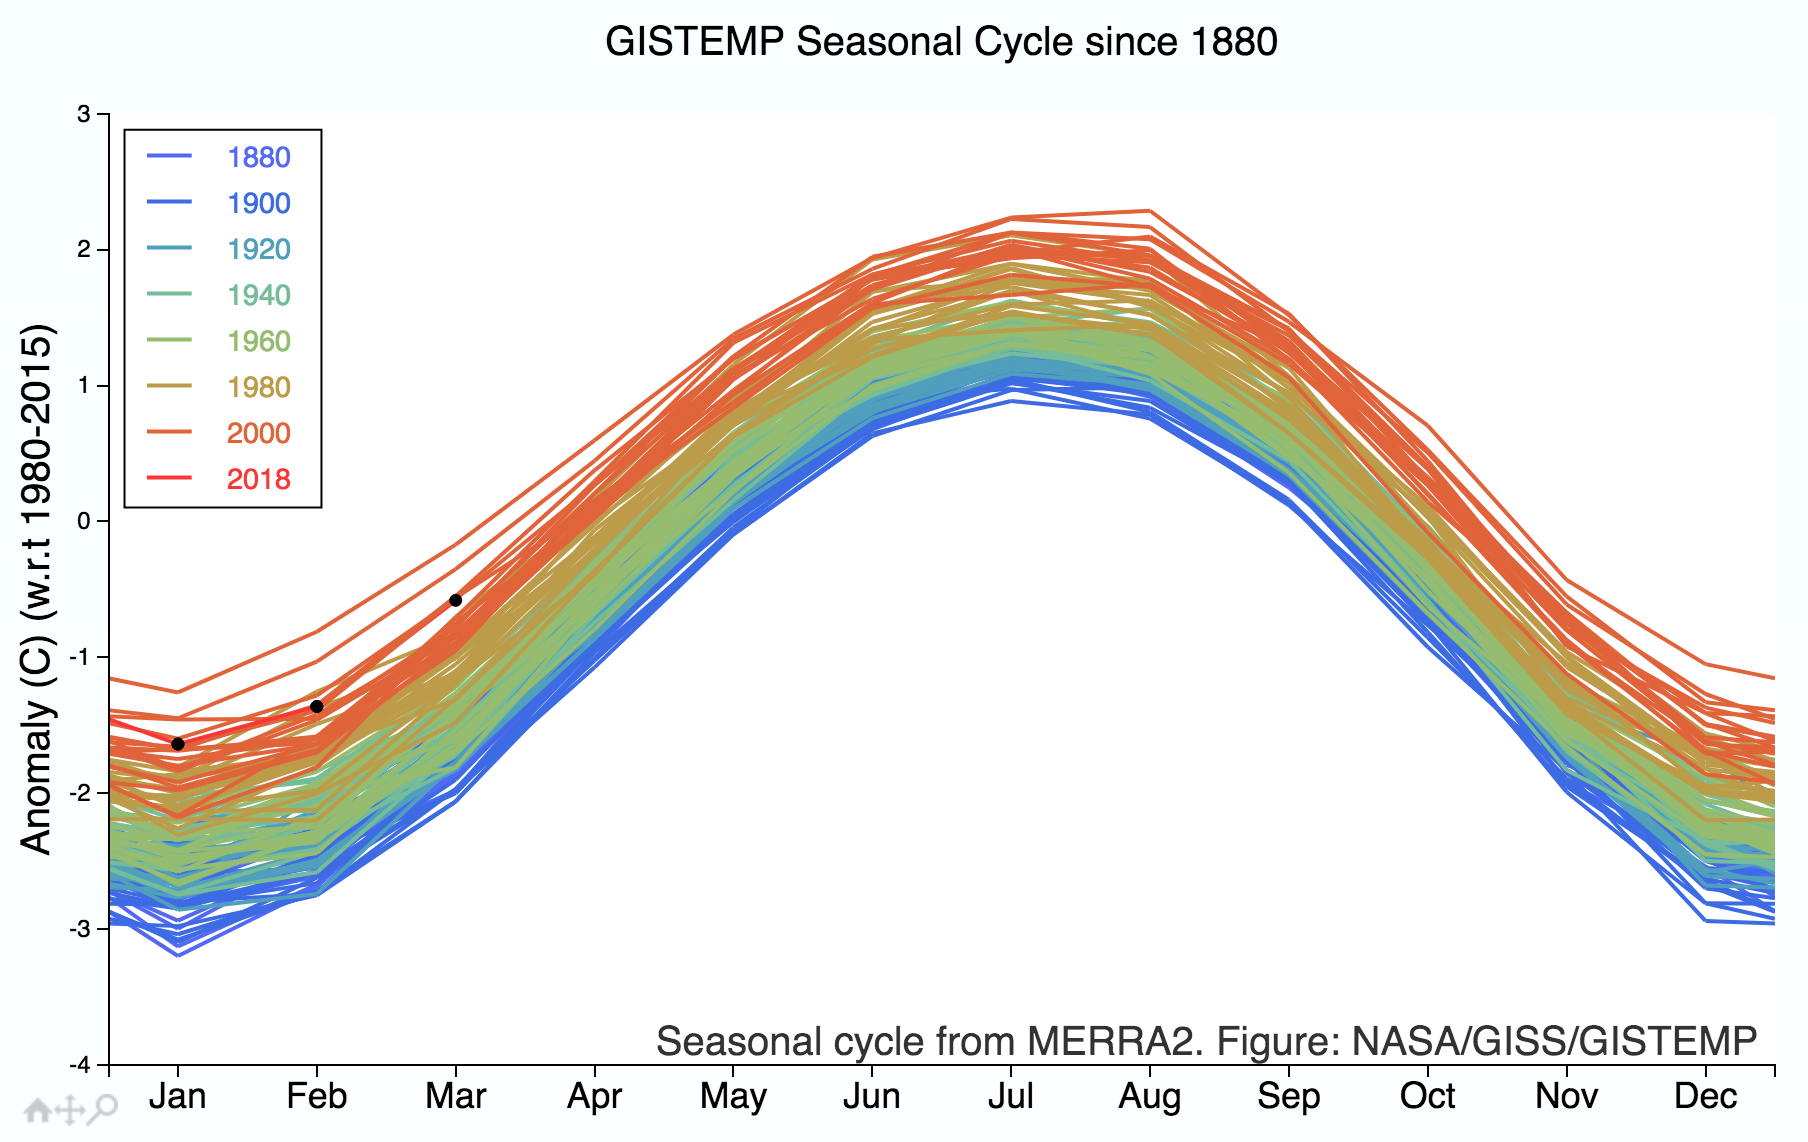
\includegraphics[width=9cm]{Grafik/GISTEMP.png} \\
	\textit{Historischer Temperaturverlauf der globalen Umgebungstemperatur über das Jahr. Es wird die Differenz zu einem jährlichen globalen Mittel dargestellt.  \\
	Quelle: \url{https://data.giss.nasa.gov/gistemp/graphs/}}
	\end{center}	
	
	(Auch könnte man sich einen Zusammenhang zwischen Fluss und Temperatur überlegen und so \(T_0\) abhängig von \(q\) machen.)
	
	Für eine genauere Aussage über die lokalen Temperatur könnte das Modell in \(n\) Behälter (anstatt nur 2) gegliedert werden, welche jeweils mit ihren Nachbarn über einen Fluss Temperatur und Salzgehalt austauschen.
	
	\newpage
	\subsection*{Anhang}
	
	Für ein besseres Verständnis des Modelles haben wir in einer ersten Studie die 6 verschiedenen Fälle von \(\alpha, \beta \) und \(\alpha - \beta\) betrachtet. Dabei wurden jeweils nur die Konstanten \(T^*_{01}, T^*_{02}\) und \(S^*_{01}, S^*_{02}\) variiert. Für die restlichen Konstanten wurden folgende Werte benutzt: \(k_T = 1, k_S = 0.1 \Rightarrow \gamma = 0.1\) und \(a = b = c = 1 \). 
	
	\begin{center}
	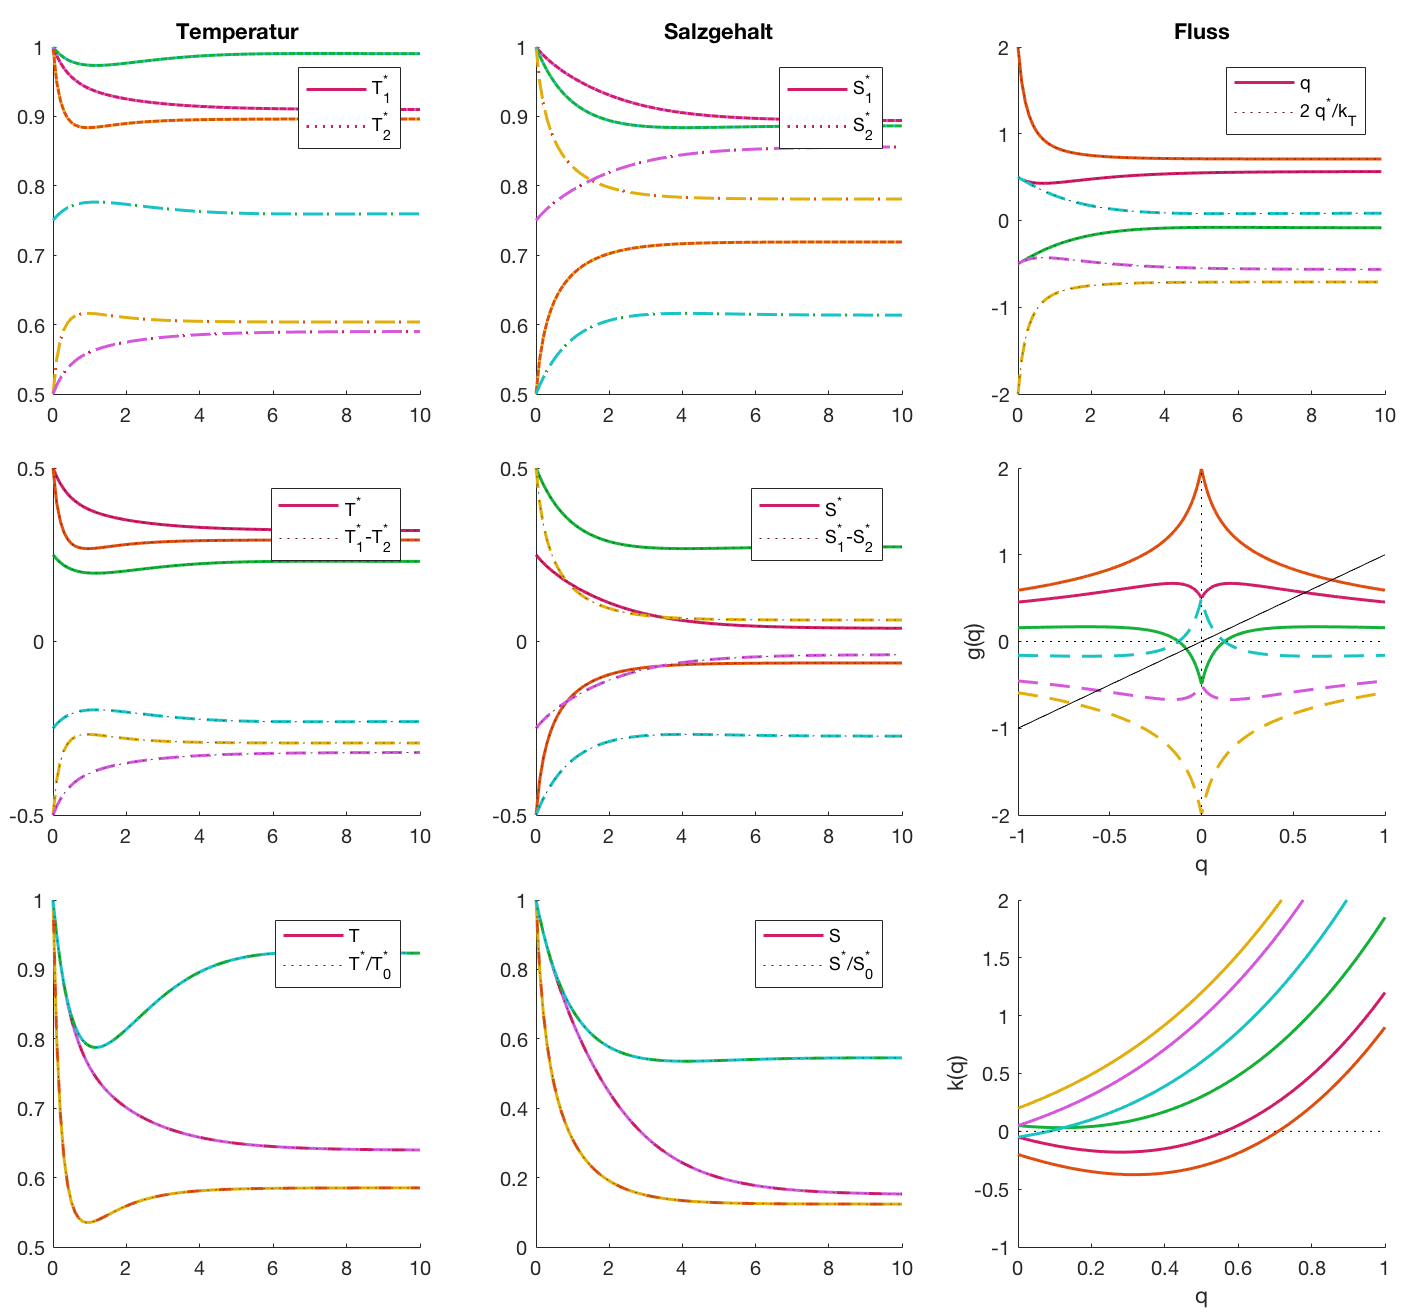
\includegraphics[width=14cm]{Grafik/Fallstudie.png}
	\begin{align*}
		\textrm{Fall 1: } &\qquad \alpha > \beta > 0: g(0) = \alpha - \beta > 0 &\qquad \footnotesize{\textrm{(rot, durchgezogen)}} \\
		&\qquad T^*_{01} = 1, T^*_{02} = 0.5, S^*_{01} = 1, S^*_{02} = 0.75 \Rightarrow \alpha = 1, \beta = 0.5 \\
		\textrm{Fall 2: } &\qquad \beta > \alpha > 0: g(0) = \alpha - \beta < 0 &\qquad \footnotesize{\textrm{(grün, durchgezogen)}} \\
		&\qquad T^*_{01} = 1, T^*_{02} = 0.75, S^*_{01} = 1, S^*_{02} = 0.5 \Rightarrow \alpha = 0.5, \beta = 1 \\
		\textrm{Fall 3: } &\qquad \alpha > 0 > \beta: g(0) = \alpha - \beta > 0 &\qquad \footnotesize{\textrm{(orange, durchgezogen)}} \\
		&\qquad T^*_{01} = 1, T^*_{02} = 0.5, S^*_{01} = 0.5, S^*_{02} = 1 \Rightarrow \alpha = 1, \beta = -1 \\
		\textrm{Fall 4: } &\qquad \beta > 0 > \alpha: g(0) = \alpha - \beta < 0 &\qquad \footnotesize{\textrm{(gelb, gestrichelt)}} \\
		&\qquad T^*_{01} = 0.5, T^*_{02} = 1, S^*_{01} = 1, S^*_{02} = 0.5 \Rightarrow \alpha = -1, \beta = 1 \\
		\textrm{Fall 5: } &\qquad \alpha < \beta < 0: g(0) = \alpha - \beta < 0 &\qquad \footnotesize{\textrm{(lila, gestrichelt)}} \\
		&\qquad T^*_{01} = 0.5, T^*_{02} = 1, S^*_{01} = 0.75, S^*_{02} = 1 \Rightarrow \alpha = -1, \beta = -0.5 \\
		\textrm{Fall 6: } &\qquad \beta < \alpha < 0: g(0) = \alpha - \beta > 0 &\qquad \footnotesize{\textrm{(türkis, gestrichelt)}} \\
		&\qquad T^*_{01} = 0.75, T^*_{02} = 1, S^*_{01} = 0.5, S^*_{02} = 1 \Rightarrow \alpha = -0.5, \beta = -1
	\end{align*}
	\end{center}		
	
	Es fällt auf, dass jeweils die Fälle 1,5 (rot,lila) sowie 2,6 (grün,türkis) und 3,4 (orange,gelb) jeweils symmetrisch zueinander stehen. Die Bedingungen des Golfstroms  ( \(T^*_1 > T^*_2, S^*_1 < S^*_2\)) erfüllt aber nur der Fall 3.

\end{document}